\documentclass[11pt, aspectratio=169, table]{beamer}
  % papersize={16cm,9cm},

\mode<presentation>{}

%%%%%%%%%%%%%%%%%%%%%%%%%%%%%%
% load packages
% add packages if needed

%\usepackage[T1]{fontenc}
\usepackage[utf8]{inputenc}
\usepackage{xcolor}
\usepackage[english]{babel}
\usepackage{amsmath,amsfonts,amssymb,amsthm}
\usepackage{color}
\usepackage[tracking=smallcaps, letterspace=-55]{microtype} % package for font spacing
\usepackage[outline]{contour}
%\usepackage[perpage]{footmisc}
\usepackage{transparent} % for setting opacity of pictures
\usepackage{pifont} % for checkmark (\ding{51}) and cross (\ding{55})
\usepackage{booktabs,array} % for tables
\usepackage{graphicx} % for figures
\usepackage{tikz}
\usepackage{pgfpages}
\usepackage{ulem}
\usepackage{dirtytalk}
\usepackage{minted}
\usepackage{textcomp}
\usepackage{mwe}
\usepackage{enumitem}

\usemintedstyle{emacs}
\setminted{fontsize=\footnotesize,python3=true}
\definecolor{bg}{rgb}{0.97,0.97,0.95}
\setmintedinline{bgcolor=bg}
\setminted{bgcolor=bg}

%\graphicspath{} % to set the path of figures

\usetikzlibrary{shapes.multipart,positioning,matrix,external,shadows}

\renewcommand{\thefootnote}{\fnsymbol{footnote}}
\renewcommand{\thempfootnote}{\fnsymbol{mpfootnote}}

%\setbeameroption{show notes on second screen=bottom}

%%%%%%%%%%%%%%%%%%%%%%%%%%%%%%
% Fill in the following information: AUTHOR, TITLE, DATE

\author[Saska Dönges]{Saska Dönges}
\title[C++ performance]{Performance considerations}
\subtitle{}
\date{March 25. 2025, BSCS2011}%{\today}
\institute{Dept.\ of Computer science, University of Helsinki
}

%%%%%%%%%%%%%%%%%%%%%%%%%%%%%%
% set beamer colors

\definecolor{hyblue}{RGB}{0,155,255}
\setbeamercolor{alerted text}{fg=hyblue}
\setbeamercolor{structure}{fg=hyblue}

\setbeamertemplate{itemize item}{\color{hyblue}}

%%%%%%%%%%%%%%%%%%%%%%%%%%%%%%
% set font (helvetica plays the role of Arial)
\usepackage{helvet}
\renewcommand{\familydefault}{\sfdefault}

%%%%%%%%%%%%%%%%%%%%%%%%%%%%%%
% set frametitle

\setbeamercolor{frametitle}{fg=black}%{fg=hyblue}
\setbeamerfont{frametitle}{series=\bfseries, shape=\scshape, size=\huge}
\setbeamertemplate{frametitle}[default][left,leftskip=3.5cm] % left shift of frame title
\addtobeamertemplate{frametitle}{\vspace{0.5cm}}{\vspace{1cm}} % spacing above and below frame title

%%%%%%%%%%%%%%%%%%%%%%%%%%%%%%
% set footline and headline
\beamertemplatenavigationsymbolsempty
\setbeamertemplate{headline}{ }
\setbeamertemplate{footline}{%
	 \usebeamercolor[fg]{page number in head/foot}%
	 \usebeamerfont{page number in head/foot}%
	\hspace{0.5cm}	
	
\includegraphics[width=2.5cm]{HY__LC05_txt__L_3L_B3____BW_cropped}
	\hfill
	\insertshorttitle\ /\ \insertshortauthor	\hfill
	\insertdate	\hspace{0.5cm}
	\insertframenumber\,/\,\inserttotalframenumber \hspace{0.5cm} \vskip2pt%
}

%%%%%%%%%%%%%%%%%%%%%%%%%%%%%%
% Other style settings
\useinnertheme{circles}

%%%%%%%%%%%%%%%%%%%%%%%%%%%%%%
% For video
\usepackage{media9}%
\newcommand{\includemovie}[3]{%
\includemedia[%
width=#1,height=#2,%
activate=onclick,%
deactivate=pageclose,%
addresource=#3,%
flashvars={%
src=#3 % same path as in addresource!
%&autoPlay=true % default: false; if =true, automatically starts playback after activation (see option ‘activation)’
&loop=true % if loop=true, media is played in a loop
&controlBarAutoHideTimeout=0 %  time span before auto-hide
}%
]{}{StrobeMediaPlayback.swf}%
}

%%%%%%%%%%%%%%%%%%%%%%%%%%%%%%
%%%%%%%%%%%%%%%%%%%%%%%%%%%%%%

\begin{document}

%% Title slide with HY picture
%{
%\usebackgroundtemplate{
%\setlength{\unitlength}{1cm}
%\begin{picture}(16,9)
%\transparent{0.33}
%\put(0.3,0.8){\includegraphics[width=15cm,height=7.8cm]{hy_brand_image_1_wide_background_hires_logo} }
%\end{picture}
%}
%\setbeamertemplate{headline}{ }%
%\begin{frame}{}
%\vspace{2.5cm}
%\begin{center}
%\huge
%{\bf \inserttitle } \\
%{\large \insertauthor}
%\end{center}
%\end{frame}
%}



% Title page without picture
{
\usebackgroundtemplate{
\setlength{\unitlength}{1cm}
\begin{picture}(16,9)
	\put(-0.1,5){ \includegraphics[width=4cm]{HY__LA01_Flame_____B3____BW} }
\end{picture}
\setlength{\unitlength}{1pt}
}
\setbeamertemplate{headline}{ }%
\begin{frame}[noframenumbering]{}
\vspace{2.5cm}
\begin{center}
\huge
\textcolor{hyblue}{ \bf
\inserttitle
} \\
{\large
\insertauthor}
\end{center}
\end{frame}
}
%

%%%%%%%%%%%%%%%%%%%%%%%%%%%%%%
%% Main text

%% set HY Logo on the upper-left corner:
\usebackgroundtemplate{
\setlength{\unitlength}{1cm}
\begin{picture}(16,2.5)
\put(0.1,0){
\includegraphics[width=2.5cm]{HY__LA01_Flame_____B3____BW}\hfill
}
\end{picture}
\setlength{\unitlength}{1pt}
}
%%

%%%%%%%%%%%%%%%%%%%%%%%%%%%%%%
%% Modify text below

\begin{frame}{After this lecture you should...}
have some idea about what goes into practical performance
\end{frame}

\begin{frame}{Agenda}
\setlength\parskip{\fill}
\tableofcontents
\alert{Interrupt} to comment or ask questions! You will get \alert{points}!
\end{frame}

\section{Instruction cycle}
\begin{frame}{Fetch--Decode--Execute -loop\footnote{\url{https://en.wikipedia.org/wiki/Instruction_cycle}}}
\setlength{\parskip}{\fill}
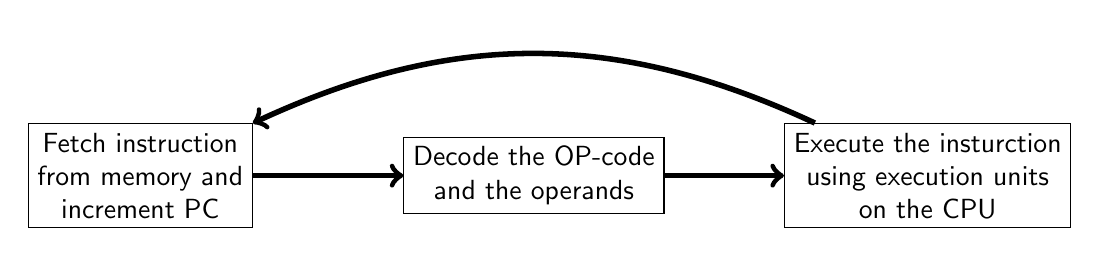
\begin{tikzpicture}
\node[rectangle, draw, align=center] at (0, 0) (Fetch) {\alert{Fetch} instruction\\from memory and\\increment PC};
\node[rectangle, draw, align=center] at (5, 0) (Decode) {\alert{Decode} the OP-code\\and the operands};
\node[rectangle, draw, align=center] at (10, 0) (Execute) {\alert{Execute} the insturction\\using execution units\\on the CPU};
\draw[->, line width=2] (Fetch) -- (Decode);
\draw[->, line width=2] (Decode) -- (Execute);
\draw[->, line width=2] (Execute) edge[bend right=25] (Fetch);
\end{tikzpicture}

Why is this something you should know as a systems programmer?

\pause
Because all (single thread) computation ``behaves'' like this. (Unless there are hardware bugs
\footnote<2->{\url{https://en.wikipedia.org/wiki/Spectre_(security_vulnerability)}})
\end{frame}

\begin{frame}{Fetch--Decode--Execute -loop}
\setlength{\parskip}{\fill}
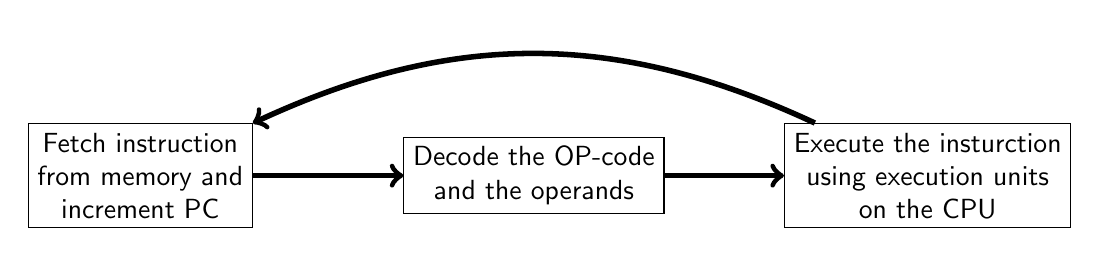
\begin{tikzpicture}
\node[rectangle, draw, align=center] at (0, 0) (Fetch) {\alert{Fetch} instruction\\from memory and\\increment PC};
\node[rectangle, draw, align=center] at (5, 0) (Decode) {\alert{Decode} the OP-code\\and the operands};
\node[rectangle, draw, align=center] at (10, 0) (Execute) {\alert{Execute} the insturction\\using execution units\\on the CPU};
\draw[->, line width=2] (Fetch) -- (Decode);
\draw[->, line width=2] (Decode) -- (Execute);
\draw[->, line width=2] (Execute) edge[bend right=25] (Fetch);
\end{tikzpicture}

Why is this not something you should concern yourself with?

\pause
Because \alert{no} modern systems \alert{actually} work like this.
\end{frame}

\begin{frame}{Why the instruction loop is a lie}
\pause
\begin{itemize}
\item \alert{Out-of-order execution} \url{https://en.wikipedia.org/wiki/Out-of-order_execution}
\item \alert{Pipelining} \url{https://en.wikipedia.org/wiki/Instruction_pipelining}
\item \alert{Speculative execution} \url{https://en.wikipedia.org/wiki/Speculative_execution}
\item \alert{Data dependence} \url{https://en.wikipedia.org/wiki/Data_dependency}
\item \alert{Cache misses} \url{https://en.wikipedia.org/wiki/CPU_cache}
\item \alert{Dark silicon} \url{https://en.wikipedia.org/wiki/Dark_silicon}
\item \alert{Variable CPI} \url{https://en.wikipedia.org/wiki/Cycles_per_instruction}
\end{itemize}
\end{frame}

\section{Memory hierarchy}
\begin{frame}{Memory hierarchy}
\setlength{\parskip}{\fill}
What is it?

What are the parts?

How fast are the parts?

Why should \alert{you} care?
\end{frame}

\begin{frame}{Teemu's Cheesecake\footnote{\url{https://www.cs.helsinki.fi/u/kerola/tikra/s2001/luennot/ch4.3_p2.pdf}}
\footnote{\url{https://en.wikipedia.org/wiki/Memory_hierarchy}}}
Relative speed differences within the memory hierarchy, compared to the differences in speed of adding the cheese to you mixing bowl when making cheesecake.

\begin{description}[style=standard,leftmargin=*]
\item{\alert{Data in register: }} Cheese already in mixing bowl $\Leftrightarrow$ Instant.
\item{\alert{Data in L1 cache: }} Cheese on spatula, ready to drop in $\Leftrightarrow$ Imperceptible slowdown.
\item{\alert{Data in L2 cache: }} Cheese on table next to bowl $\Leftrightarrow$ Often irrelevant an unavoidable.
\item{\alert{Data in LL cache: }} Chesee in fridge $\Leftrightarrow$ Slightly annoying but you have to get it at some point.
\end{description}
\end{frame}

\begin{frame}{Teemu's Cheesecake}
\begin{description}[leftmargin=*]
\item{\alert{Data in RAM: }} You forgot to buy cheese $\Leftrightarrow$ Put stuff away and continue when you get back from the store.
\item{\alert{Data on SSD: }} Global supply chain shortage $\Leftrightarrow$ Cheese will be available in some days.
\item{\alert{Data on Spinning disk: }} Cheese on the ISS $\Leftrightarrow$ Talk to NASA, perhaps available in some months.
\item{\alert{Access requires human intervention: }} Cheese on the moon $\Leftrightarrow$ No planned missions, technically possible in a couple of years.
\end{description}

Fortunately computers are very patient.
\end{frame}

\begin{frame}{Why care about the cheesecake?}
\setlength{\parskip}{\fill}
Unless your computation happens almost entirely in registers and low level cache, memory access latencies 
will probably have a \alert{massive} effect on practical performance!

Fortunately, modern hardware is \alert{amazing} at hiding memory latency, if your memory access patterns
are ``\alert{predictable}''.

Unfortunately only the engineers at Intel and AMD, know exactly what ``predictable'' means.

This should be a central topic at the case study session next week.
\end{frame}

\section{Division}
\begin{frame}{Division}
\setlength\parskip\fill
Is division bad? 

Should you care?

When?

Why? / Why not?
\end{frame}

\begin{frame}[fragile]{Division by constant is ok}
If you use an optimizing compiler, any division by a constant will be fine.

\begin{minted}{cpp}
uint32_t div_by(uint32_t x) {
    return x / 310;
}
\end{minted}

\begin{minted}{asm}
mov     eax, 3546811703
mov     ecx, edi
imul    rax, rcx
shr     rax, 40
ret
\end{minted}
\end{frame}

\begin{frame}[fragile]{Division by something unknown sucks}
If you just have to divide, you have to pay the price.

\begin{minted}{cpp}
std::pair<uint64_t, uint64_t> div_by(uint64_t x, uint64_t a) {
    return {x / a, x % a};
}
\end{minted}

Upside is that \texttt{mod} is free if you \texttt{div}.

\begin{minted}{asm}
mov     rax, rdi
xor     edx, edx
div     rsi
ret
\end{minted}
\end{frame}

\begin{frame}[fragile]{Practical take-aways}
\setlength\parskip\fill
Use \mintinline{cpp}{const} when you can, or otherwise make sure that the compiler knows the divisor is a constant.

More generally: Only optimize manually when it actually matters.

For example: Don't work a lot to eliminate branching that the compiler would eliminate anyway.

\mintinline{cpp}{if (a) x = 1; else x = 2;} vs. \mintinline{cpp}{x = a ? 1 : 2;}.
\end{frame}

\section{Loop unrolling}
\begin{frame}{Should you do loop unrolling manually}
\setlength\parskip\fill
Probably not...

Why?

What should you do then?
\end{frame}

\begin{frame}[fragile]{Compilers do \alert{very} aggressive loop unrolling}
\setlength\parskip\fill
Check if your loop gets unrolled. Unrolling has high overhead but high througput.

If it does and it shouldn't. Try to stop it. \mintinline{cpp}{[[assume]]} and \mintinline{cpp}{[[unreachable]]} perhaps?

If it should and it doesn't. Figure out why and fix it. Perhaps eliminate data dependence or manually split loops.

Typically works very well for common programming patterns, and is \alert{immensely difficult} when it doesn't.
\end{frame}

\section{Are trees bad actually?}
\begin{frame}{Trees?}
\setlength\parskip\fill
Are trees bad?

Why?

Why not?
\end{frame}

\begin{frame}{Reference-based data structures}
\setlength\parskip\fill
Reference-based data structures have a risk of spreading out over application memory, in a way that may as well be random.

Unless your use case specifically can't avoid random memory access, a purely reference-based structure is probably not for you.

Luckily, a lot of tree structures can be made more blocky, and thus more memory efficient\footnote{\url{https://en.wikipedia.org/wiki/B-tree}}.
\end{frame}

\section{Templates}
\begin{frame}{Templates, not just generics!}
\setlength\parskip\fill
Are they amazing?

Are they a 0-cost abstration\footnote{\url{https://youtu.be/rHIkrotSwcc}}?

Should you do everything you possibly can with templates?
\end{frame}

\begin{frame}{Template everything?}
\setlength\parskip\fill
From a purely \alert{PfP} point of view... Kinda yes... If you don't mind hard-to-maintain code... And as long as you don't run 
into insurmountable issue w.r.t compile time or binary size.

Templating kinda either eliminates branching or moves it lower on the call stack.

So the main benefit is less issues with branch missprediction? Right?

\pause
Not really. Well written code will have very few unavoidable branch misspredictions anyway. 

But templating can improve the working of the instruction cache massively, which is often a more important thing, than a simple missed branch.
\end{frame}

\section{How to know what to do}
\begin{frame}{How should I know what is or isn't fast in practice?}
\setlength{\parskip}{\fill}
\pause
\alert{Figure it out!}
\begin{itemize}
\item Look it up online.
\item See what compiler produces.
\item Run profiling (cachegrind, grpof...).
\item Run actual michrobenchmarks.
\item Remain skeptical of everything. 
\end{itemize}
\end{frame}

%{
%\usebackgroundtemplate{
%\transparent{0.3} % requires \usepackage{transparent} & compile twice
%\setlength{\unitlength}{1cm}
%\begin{picture}(16,9)
%\put(0.2,1){
%\includegraphics[width=15cm,height=7.5cm]{hy_brand_image_1_wide_background_hires_logo}
%}
%\end{picture}
%\setlength{\unitlength}{1pt}
%}
%
%\begin{frame}{\vspace{3cm}That's it}
%\begin{center}
%\vspace{-4cm}{\huge Questions?}
%\end{center}
%\end{frame}
%}

\end{document}
